\section{Tagging} \label{sc:Tagging}
The tagging part of the system is one of the primary elements of the system. The implementation of the concept consists of multiple parts, such as creating and maintaining the tags, attaching tags to assets, and searching through assets based on tags.
\par
Most of these parts have not been included in this section, because they are easily implemented or trivial. The parts chosen for this section are the handling of users, connections between multiple tags, connections to departments, and the attachment of tags to assets and the effects of this.

\subsection{Users as tags}
To make it possible to attach users to assets, the \textit{User} class implements the \textit{ITagable} interface. This interface is defined to allow lists to contain both tags and users. By referring to an abstraction they both implement, it is possible to avoid specifically addressing either tags or users. 
\par
The interface demands the implementing classes to contain all the attributes related to a tag. This makes it possible to handle users and tags the same way in situations such as attaching users and tags to an asset or searching the assets based on attached users and tags.

\subsection{Parent-child and department relation}
To better organize tags, each tag belong to one or all departments. This will decrease the number of tags being shown in the suggestions across the application and will make it easier for the user to find the right tag. If a tag belongs to all departments, it will appear no matter the current department of the user.
\par
Separating the tags into departments improves the overall simplicity of the system, but a single department can still end up containing a large amount of tags. To further divide the tags, and ease the task of finding the right tag, a hierarchical structure has been implemented through parent tags.
\par
Every tag belongs to one or all departments, but by the introduction of parent tags, they can also belong to another tag. This way, fields, color, and the department of a tag can be inherited by other tags. This also makes it easier to create multiple tags with the same fields.
\par
The hierarchic structure of the tags and departments only has three levels, as a parent tag cannot belong to another parent tag (see \autoref{fig:TagHierarchicStructureWithDepartment}).

\begin{figure}[H]
    \centering
    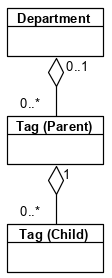
\includegraphics[width=0.18\textwidth]{figures/Implementation/TagHierarchicStructure.png}
    \caption{The hierarchic structure of the parent-child relation of tags. If a tag has no department, it belongs to all departments.}
    \label{fig:TagHierarchicStructureWithDepartment}
\end{figure}

In this implementation, a tag is by default a parent tag without any children. A child tag is created by assigning a value to its \textit{ParentId}. This means that it is possible for a parent tag to have no children, but a child tag must have a parent, otherwise it will be a parent itself.
\par
The connection between the parent and its children is an aggregation. The children will get the fields, color, and department of the parent. The color can be changed, but the department is locked to that of its parent. This is done because it should not be possible to create relations between tags from different departments.
\par
Within the system, the parents and children are treated differently in a few situations. If a parent tag contains children, only the children can be attached to an asset. However, if a parent tag does not contain children, the parent tag can be attached.

\subsection{Asset-tag relation}
Attaching tags to assets is the main purpose of the tags. When a tag is attached to an asset, the asset gets the fields from the tag, and an instance of the \textit{Asset-tag relation} class (see \autoref{fig:ModelComponentClassDiagram}) is generated. This class, however, has not been implemented in the system but exists in the database as two relational tables. The first table contains relations between the asset and tag tables and the second contains relations between the asset and user tables (see \autoref{app:database_diagram}). 
\par


For simplicity, only the table connecting the asset and tag tables have been described, but the same principles apply to the relation between the asset and user tables. The reason for having two different tables is that a tag and a user can both have the same database ID, which could cause issues if they were placed in the same table.
\par
A row in the relational table contains the IDs of the asset and a tag attached to it (see \autoref{app:database_diagram}, table asset\_tags). When fetching either assets or tags, the table can be used to get all the objects of one connected to a specific instance of the other. This relational table also makes it possible to have a single tag attached to multiple assets, without copying the tag to every. By this, keeping the relational table up to date, even if either the tag or the asset is updated.
\par
This relational table also ensures that fields attached to a tag can be added to the assets with the given tag when they are opened for editing. The fields could be added as soon as the tag is updated, but if the tag is attached to hundreds of assets, the value of the field would potentially have to be set for all these assets.
\par
Adding or removing a tag from an asset is as simple as adding or removing a row in the relational table. If the assets were connected to tags directly, the removal of a tag would demand every asset connected to the tag to be updated, which would be a resource intensive operation.
\par
The relational table also makes it possible to search for assets based on the tags attached to them. This makes it easier to find assets and gives the opportunity to filter the assets based on attached users and tags.
\par
The primary advantage of using a relational table is that the data will only exist once throughout the database and updating an entry will only have to be done once. The biggest problem of the relational table is its increase to run time as the database grows. The increase in execution time is caused by the fact that the table must be iterated through to find the correct relation. However, this has been improved by using an index, which maps the search to the table and removes the need to iterate through every entry \citep{RelationalTable}.
\par




A good example of the use of the relational tables is the method in \textit{AssetRepository} that attaches tags and users to an asset (see \autoref{code:AssetRepositoryAttachTags}). This method takes in an asset and a list of \textit{ITagable}s. This way, the method can simply be called once and all the asset-tag and asset-user relations are created. Because the tags and users are in two different tables, and both could be in the input list, the method has to check which table each connection should be placed in, and inserts it. 
\par
Lines \ref{lines:AssetRepUserList} and \ref{lines:AssetRepTagList} in \autoref{code:AssetRepositoryAttachTags} creates a list of \textit{Users} and \textit{Tags} from the single list of \textit{ITagable}s.
Then an SQL query, specifying that the following values should be inserted into the asset-users table, is created. Then in lines \ref{line:AssetRepUserForLoopBegin} to \ref{line:AssetRepUserForLoopEnd} is a for-loop that iterates over the list of \textit{Users}, adding the id's of the users and the asset to the query. 
\par
The same process is repeated for the list of \textit{Tags} in lines \ref{line:AssetRepTagForLoopBegin} to \ref{line:AssetRepTagForLoopEnd}, where the id's are inserted into the asset\_tags table (see \autoref{app:database_diagram}).

\begin{listing}[H]
\begin{minted}[frame=lines, framesep=3mm, baselinestretch=1, linenos, bgcolor=LightGray, escapeinside='', breaklines]{csharp}
public bool AttachTags(Asset asset, List<ITagable> listOfTags)
{
    ...
        
    List<User> users = listOfTags.OfType<User>().ToList(); '\label{lines:AssetRepUserList}'
    List<Tag> tags = listOfTags.OfType<Tag>().ToList(); '\label{lines:AssetRepTagList}'
    int userCounter = users.Count;
    int tagCounter = tags.Count;
        
     ...

    StringBuilder userQuery = new StringBuilder("INSERT INTO asset_users VALUES ");

    for (int i = 0; i < userCounter; i++) '\label{line:AssetRepUserForLoopBegin}'
    {
        userQuery.AppendFormat("({0},{1})", asset.ID, users[i].ID);

        if (i != userCounter - 1)
            userQuery.Append(",");
    } '\label{line:AssetRepUserForLoopEnd}'

    StringBuilder tagQuery = new StringBuilder("INSERT INTO asset_tags VALUES ");

    for (int i = 0; i < tagCounter; i++) '\label{line:AssetRepTagForLoopBegin}'
    {
        tagQuery.AppendFormat("({0},{1})", asset.ID, tags[i].ID);
        
        if (i != tagCounter - 1)
            tagQuery.Append(",");
    }'\label{line:AssetRepTagForLoopEnd}'
            
    ...
       
    return querySuccess;
}
\end{minted}
\captionof{listing}{AssetRepository AttachTags method}
\label{code:AssetRepositoryAttachTags}
\end{listing}